\chapter{植被水力模式}
%\addcontentsline{toc}{chapter}{植被水力模式}

%\begin{植被水力模式}
CoLM植被水力模式根据土壤-植物-大气连通体的概念计算陆气水分交换的蒸腾分量。
CoLM植被水力模式中的植物水分传输得益于土壤、根、茎、叶和大气之间形成的水势梯度。植物各部位的水势也密切影响着各植被水力过程。
首先,根、茎、叶的水势通过植物栓塞过程影响着植物水分传输能力 (详见章节~\ref{植被水力导度的衰减})。
其次,植物根与每层土壤的水势梯度将影响根的水力重分配过程 (详见章节~\ref{地下植被水力过程})。最后,叶片的水势降低将影响叶片气孔导度,
同时影响植物水分传输和光合作用 (详见章节~\ref{气孔导度的水分胁迫})。


\section{植物水势动态}\label{植物水势动态}
植物水势的动态模拟是CoLM植被水力模式的关键。CoLM植被水力模式的水势模拟包括地上和地下植被水力过程两部分。
地上部分包括在阳叶、阴叶、茎和地表根四个节点间的水势 ($\Psi_{sun}$,$\Psi_{sha}$,$\Psi_{stem}$,$\Psi_{root,0}$)
%
 模拟;地下部分包括地表根以及$n$层地下根 $n+1$个节点的水势 ($\Psi_{root,i}$,$i=0,1,2,\ldots,n$) 模拟。地上、地下两部分通过地表根水势
 ($\Psi_{root,0}$)的模拟被密切的耦合(如图~\ref{fig:CoLM植被水力模型示意图})。

{
\begin{figure}[htbp]
\centering
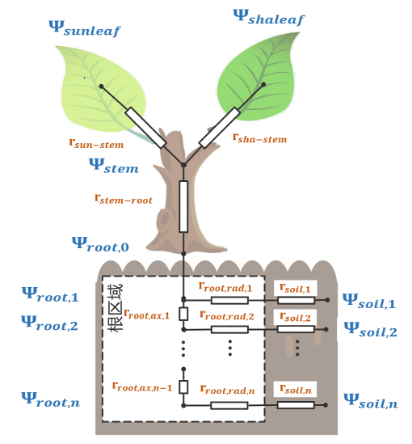
\includegraphics{Figures/植被水力模式/CoLM植被水力模型示意图.png}
\caption{CoLM植被水力模型示意图。}
\label{fig:CoLM植被水力模型示意图}
\end{figure}
}


CoLM植物水势的动态模拟假设植物水分传输为稳恒流,并将其类比为电路问题~
\citep{van1948water},即水分传输速率正比于水势差和水力导度。
地上部分四个节点的水势梯度和水通量之间的关系由Darcy定律表达,满足以下方程:
\begin{equation}\label{q_sunstem}
q_{ {sun \leftarrow stem }}=k_{{sun} \leftarrow  {stem}}\left(\Psi_{sun}-\Psi_{stem}\right)
\end{equation}
\begin{equation}
q_{ {sha \leftarrow stem }}=k_{ {sha} \leftarrow {stem}}\left(\Psi_{sha}-\Psi_{ {stem }}\right)
\end{equation}
\begin{equation}
q_{ {stem \leftarrow root }}=k_{ {stem } \leftarrow  { root }}\left(\Psi_{ {stem }}-\Psi_{ {root }, 0}\right)
\end{equation}
$k_{sun \leftarrow stem}$,$k_{sha \leftarrow stem }$,$k_{stem \leftarrow root }$ 分别代表茎到阳叶的水力导度、茎到阴叶的水力导度和根到茎的水力导度。
水力导度随水势降低而降低,是关于茎和根水势的函数 (详见章节~\ref{植被水力导度的衰减}) 。地表根水势$\Psi_{root,0}$是关于每层土壤水势 ($\Psi_{soil,i}$) 
及根总吸水速率 ($q_{root,0}$) 的函数,由地下植被水力过程所计算 (详见章节~\ref{地下植被水力过程}):
\begin{equation}\label{Psi_root_0}
\Psi_{root, 0}=R\left(\Psi_{ {soil }, i}, q_{root, 0}\right)
\end{equation}
$q_{sun \leftarrow stem}$,$q_{sha \leftarrow stem }$,$q_{stem \leftarrow root }$分别代表茎到阳叶的水流通量、茎到阴叶的水流通量和根到茎的水流通量。
水流通量在各节点由于稳恒流假设,满足水分守恒方程:
\begin{equation}
E_{sun}=q_{sun \leftarrow  stem}
\end{equation}
\begin{equation}
E_{ {sha }}=q_{ sha \leftarrow stem}
\end{equation}
\begin{equation}
q_{ {sun \leftarrow stem }}+q_{ {sha \leftarrow stem }}=q_{ {stem \leftarrow root }}
\end{equation}
\begin{equation}\label{q_stemroot}
q_{stem \leftarrow root}=q_{root, 0}
\end{equation}
$E_{sun}$代表阳叶蒸腾速率,$E_{sha}$代表阴叶蒸腾速率。它们是由无水分胁迫情况下的叶片蒸腾 ($E_{sun,max}$, $E_{sha,max}$) 
和受叶片水势 ($\Psi_{sun}$,$\Psi_{sha}$) 控制的蒸腾衰减函数所组成(详见章节~\ref{植被水力导度的衰减})。


\section{植被水力导度的衰减}\label{植被水力导度的衰减}
植物水势下降导致的空穴现象会严重降低水分在植物内部的传导能力。我们将实验上观测到水力导度随水势变化的S型脆弱性曲线 
\citep{sperry1988method,gentine2016allometry,neufeld1992genotypic,pammenter1998mathematical,plaut2012hydraulic}
 引入到模型,对植被水力栓塞进行参数化,得到节点间的水力导度$k_{i\gets j}$ (从节点$j$到$i$的传输):
\begin{equation}
k_{i \leftarrow j}=k_{max} \cdot 2^{-\left(\frac{\Psi_{\mathbf{j}}}{p 50}\right)^{c_{k}}}
\end{equation}
其中$k_{max}$表示最大水力导度 (\unit{s^{-1}})。$\Psi_j$代表节点$j$的水势 (\unit{mm.H_2O}),$p50$代表水力导度降低 50\% 时的水势 (\unit{mm.H_2O}),$c_k$代表脆弱性曲线的形状参数。


实验数据发现气孔导度和叶片水势同样存在S型曲线关系 \citep{kennedy2019implementing,klein2014variability},我们用如下方程~\eqref{Esun_psi}和~\eqref{Esha_psi}表达叶片水势降低对阳叶和阴叶的实际蒸腾速率($E_{sun}$和$E_{sha}$)的影响:
\begin{equation}\label{Esun_psi}
E_{sun}=E_{sun,max} \cdot 2^{-\left(\frac{\Psi_{\mathbf{sunleaf}}}{p 50}\right)^{c_{k}}}
\end{equation}
\begin{equation}\label{Esha_psi}
E_{sha}=E_{sha,max} \cdot 2^{-\left(\frac{\Psi_{\mathbf{shaleaf}}}{p 50}\right)^{c_{k}}}
\end{equation}
其中,$E_{sun,max}$和$E_{sha,max}$是无水分胁迫条件下的蒸腾速率,由最大气孔导度($g_{s,max}^{sun}$, $g_{s,max}^{sha}$)结合地表湍流参数化方案算出,最大气孔导度由CoLM光合气孔耦合模型($FvCB$)在无水分胁迫条件下计算得出,(最大蒸腾速率和最大气孔导度的计算详见章节~\ref{气孔导度的水分胁迫})。


\section{地下植被水力过程}\label{地下植被水力过程}
地下植被水力过程主要体现在水力重分配过程上,水力重分配描述了水分通过地下根系从湿润土壤层向干燥土壤层传输的过程。
是一个受水势梯度所驱动的生物物理过程。CoLM引入了Amenu水力重分配模型\citep{amenu2008} \citep{zhu2017incorporating},
并将地下植被水力过程和地上植被水力过程相耦合 \citep{li2021new},考虑刻画除根、茎和叶等地上节点外的, 
$n$个不同土壤深度的根系水力节点的水势动态变化 (如图~\ref{fig:CoLM植被水力模型示意图})。模式中的水力传导包括轴向水力传导和径向水力传导。

根据Darcy定律,根轴向水力传导方程为:
\begin{equation}\label{k_axi}
k_{ax,i}\left(\Psi_{r,i}-\Psi_{r,i+1}\right)=q_{ax,i}
\end{equation}
其中$k_{ax,i}$代表第$i+1$层到第i层根节点间的根轴向水力导度,$q_{ax,i}$代表相应的轴向水传输速率,
$\Psi_{r,i}$代表第$i$层根节点的水势。$i$取值1到$n-1$,$n$代表土壤总层数。\\
根径向水力传导方程为:
\begin{equation}\label{k_radi}
k_{rad,i}\left(\Psi_{soil,i}-\Psi_{r,i}\right)=q_{rad,i}
\end{equation}
其中$k_{rad,i}$代表第$i$层土壤节点到根节点间的径向水力导度,
$q_{rad,i}$代表相应的径向水分传输速率,$\Psi_{soil,i}$代表第$i$层土壤节点的水势,$i$取值1到$n$。



对于第2到$n$层的土壤根节点存在水分平衡方程:
\begin{equation}\label{q_axi}
q_{a x, i}+q_{r a d, i}=q_{a x, i-1}
\end{equation}
其中$i=2, \ldots, n$,方程~\eqref{q_axi} 实际上是$n-1$个方程组。


另外,由表层根节点和地上植物水力网络构成的水分平衡关系,可得:
\begin{equation}\label{q_ax1}
q_{ax,1}+q_{rad, 1}=q_{root,0}
\end{equation}
将方程~\eqref{k_axi}和~\eqref{k_radi}代入~\eqref{q_axi}和~\eqref{q_ax1},则得到关于$ \Psi_{r,i}$的$n$个线性方程组。
这$n$个线性方程组描述了在植物地下水力网络中,根水势的动态变化。CoLM地下植被水力过程的输入包括土壤水势垂直分布 ($\Psi_{soil,i}$)和根总吸水速率 ($q_{root,0}$),输出包括根水势垂直分布($\Psi_{r,i}$)和根吸水速率的垂直分布 ($q_{rad,i}$)。因此,地下植被水力过程可以概括地表达为土壤水势和总吸水速率的函数,如方程~\eqref{Psi_root_0}。


\section{气孔导度的水分胁迫}\label{气孔导度的水分胁迫}
土壤水分亏缺对植物的影响主要表现在对植被生理过程的限制,通常用水分胁迫因子来量化,CoLM中的水分胁迫因子作为取值 $0\sim 1$ 的无量纲变量,限制气孔导度和光合羧化能力,见公式~\eqref{V_cmaxsun_a}--~\eqref{R_d1_sha}。

植被水力模式关闭时(土壤水分胁迫方案SMS),水分胁迫因子 ($\beta$) 取决于根的垂直分布比例和土壤水势:
\begin{equation}\label{beta_0}
\beta=\sum_{i=1}^{n} froot_i \beta_{i}
\end{equation}

\begin{equation}\label{beta_i}
\beta_{i}=\frac{\Psi_{\max }-\Psi i}{\Psi_{\max }-\Psi_{s a t}}
\end{equation}
$froot_i$是第i层土壤中根的比例,$\beta_i$是第$i$层土壤的水分胁迫因子贡献;它由每层土壤的实际水势 (${\Psi}_i$),最大水势 (${\Psi}_{max}$)和饱和水势 (${\Psi}_{sat}$)计算得出。

当植被水力模式开启时(植被水力方案PHS),植物叶水势($\Psi_{\mathbf{sunleaf}}$,$\Psi_{\mathbf{shaleaf}}$)的降低直接造成植物水分胁迫,从而导致气孔关闭以保持植物茎的导水能力。
气孔这一行为符合植物生理学理论,水分胁迫因子按阴叶和阳叶区分,由气孔导度($\beta_{sun}$,$\beta_{sha}$)的衰减比例来定义:
\begin{equation}\label{beta_sun}
\beta_{sun}=\frac{g_{s}^{sun}}{g_{s,max}^{sun}}
\end{equation}
\begin{equation}\label{beta_sha}
\beta_{sha}=\frac{g_{s}^{sha}}{g_{s,max}^{sha}}
\end{equation}
$g_{s}^{sun}$和$g_{s}^{sha}$分别为阳叶和阴叶实际的气孔导度,$g_{s,max}^{sun}$和$g_{s,max}^{sha}$分别为阳叶和阴叶无水分胁迫条件下的气孔导度。其计算从无水分胁迫条件出发($\beta_{sun}=1$, $\beta_{sha}=1$),应用光和气孔耦合模型($FvCB$),计算得出无水分胁迫条件下的气孔导度。光合气孔耦合模型($FvCB$)由气孔导度经验模型~\eqref{ei_cssun}和~\eqref{ei_cssha},气体扩散方程~\eqref{ci_1sun}和~\eqref{ci_1sha},和Farquhar光合作用模型~\eqref{An1sun}和~\eqref{An1sha}联立而成,气孔导度是该模型重要的输出变量:
\begin{equation}\label{gs_sunmax}
g_{s,max}^{sun}=FvCB\left(\beta_{sun}=1\right)
\end{equation}
\begin{equation}\label{gs_shamax}
g_{s,max}^{sha}=FvCB\left(\beta_{sha}=1\right)
\end{equation}


相应地,最大蒸腾速率($E_{sun,max}$和$E_{sha,max}$)可由最大气孔导度结合地表冠层湍流参数化方案~\eqref{Ev}在阳叶和阴叶上分别计算得出 (如图~\ref{fig:光合气孔模式和植被水力模式的耦合示意图})。

\begin{equation}\label{E_sunmax}
E_{sun,max}=\rho_{atm} c_{vsun,max}^{w} \cdot \frac{c_{a}^{w} q_{atm}+c_{g}^{w} q_{g}-
\left(c_{a}^{w}+c_{g}^{w}\right) q_{s a t}^{T_{v}}}{c_{a}^{w}+c_{g}^{w}+c_{vsun,max}^{w}+c_{vsha,max}^{w}}
\end{equation}
%
\begin{equation}\label{Eshamax}
E_{sha,max}=\rho_{atm} c_{vsha,max}^{w} \cdot \frac{c_{a}^{w} q_{atm}+c_{g}^{w} q_{g}-
\left(c_{a}^{w}+c_{g}^{w}\right) q_{s a t}^{T_{v}}}{c_{a}^{w}+c_{g}^{w}+c_{vsun,max}^{w}+c_{vsha,max}^{w}}
\end{equation}


$cf$为导度的单位转换系数(\unit{umol.m^{-3}}),将\unit{umol.m^{-2}.s^{-1}}转换为\unit{m.s^{-1}}。$c_{vsun,max}^{w}$和$c_{vsha,max}^{w}$是阳叶和阴叶的最大冠层导度,即无植被水分胁迫条件下的冠层导度,可表达为最大气孔导度的函数,如公式~\eqref{cvsun_gsmax}和~\eqref{cvsha_gsmax}:
\begin{equation}\label{cvsun_gsmax}
    c_{vsun,max}^{w}=\left(1-f_{wet}\right)\frac{f_{sun}\text{LAI}}{cf\left(\frac{1}{g_b}+\frac{1}{g_{s,max}^{sun}}\right)}
\end{equation}
%
\begin{equation}\label{cvsha_gsmax}
    c_{vsha,max}^{w}=\left(1-f_{wet}\right)\frac{f_{sha}\text{LAI}}{cf\left(\frac{1}{g_b}+\frac{1}{g_{s,max}^{sha}}\right)}
\end{equation}

结合叶水势对蒸腾的影响~\eqref{Esun_psi}和~\eqref{Esha_psi},可计算得到的实际蒸腾速率$E_{sun}$和$E_{sha}$,从地表冠层湍流参数化方案反推,可得到干阳叶和干阴叶的冠层导度 ($c_{vsun}^{w}$和$c_{vsha}^{w}$)。如公式~\eqref{cv_Esun}和~\eqref{cv_Esha}:
\begin{equation}\label{cv_Esun}c_{vsun}^{w}=\frac{E_{sun}\left(c_a^w+c_g^w+c_{v,wet}^{w}\right)}{\left(\left(c_a^w+c_g^w\right)q_{sat}-c_a^w q_m - c_g^w q_g\right)\rho-E_{sun}-E_{sha}}
\end{equation}

\begin{equation}\label{cv_Esha}
c_{vsha}^{w}=\frac{E_{sha}\left(c_a^w+c_g^w+c_{v,wet}^{w}\right)}{\left(\left(c_a^w+c_g^w\right)q_{sat}-c_a^w q_m - c_g^w q_g\right)\rho_{atm}-E_{sun}-E_{sha}}
\end{equation}
其中,$c_{v,wet}^{w}$是湿叶蒸发导度,如公式~\eqref{cwet}
\begin{equation}\label{cwet}
c_{v,wet}=\frac{f_{wet}\left(\text{LAI}+\text{SAI}\right)g_b}{cf}
\end{equation}
从干阳叶和干阴叶的冠层导度和气体扩散方程可进一步算出叶片气孔导度:
%\begin{equation}\label{gssun_cvsun}
%
%\end{equation}

耦合植被水力模式、光合气孔模式和地表冠层湍流参数化方案,再利用公式~\eqref{beta_sun}和\eqref{beta_sha}可以完整地求解植被水力模式下的植物水分胁迫 (如图 \ref{fig:光合气孔模式和植被水力模式的耦合示意图})。
{
    \begin{figure}[htbp]
    \centering
    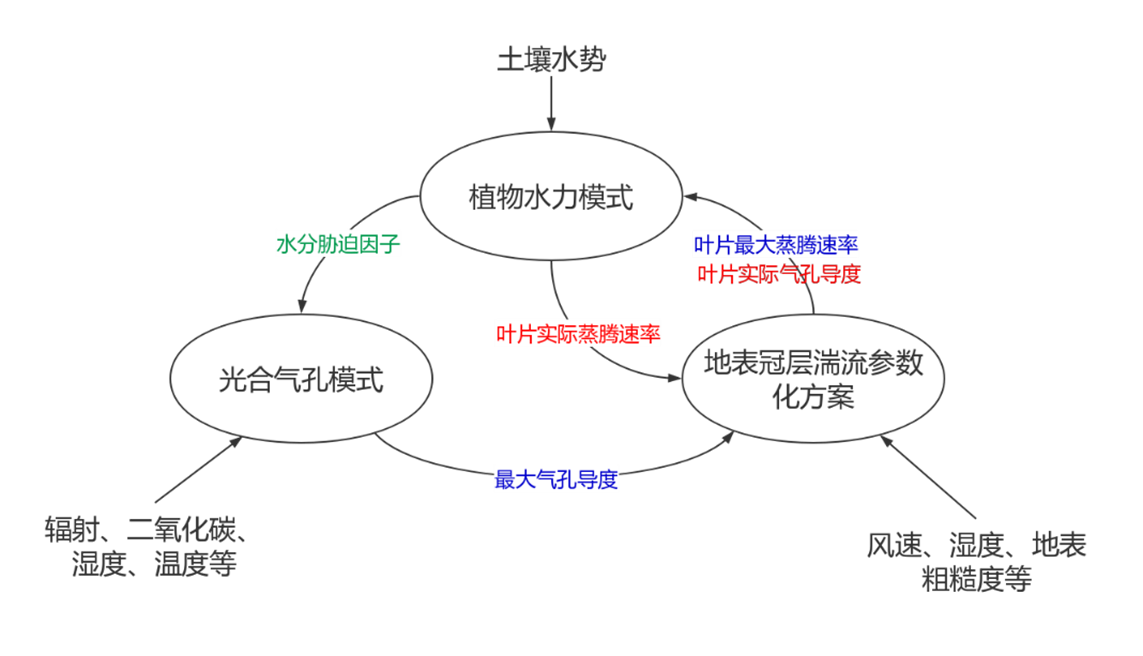
\includegraphics{Figures/植被水力模式/光合气孔模式和植被水力模式的耦合示意图.png}
    \caption{光合气孔模式和植被水力模式的耦合示意图。}
    \label{fig:光合气孔模式和植被水力模式的耦合示意图}
    \end{figure}
}


\section{数值计算方案}\label{数值计算方案}
求解植物水势、水分胁迫、气孔导度和叶片蒸腾速率,需要耦合植被水力模式、光合气孔模式和地表冠层参数化方案。
耦合描述植物水势变化的动力方程组(公式(\ref{q_sunstem})--(\ref{q_stemroot}), (\ref{Esun_psi}) 和(\ref{Esha_psi})),
地表冠层参数化方案 (公式(\ref{E_sunmax})--(\ref{cvsha_gsmax})),
光合气孔模式的最大气孔导度计算 (公式(\ref{gs_sunmax})和(\ref{gs_shamax})), 植物水分胁迫计算(公式(\ref{beta_sun})和(\ref{beta_sha})),共18个方程,
求解包括4个植物地上水势节点 ($\Psi_{sunleaf}$, $\Psi_{shaleaf}$, $\Psi_{stem}$和$\Psi_{root,0}$),8个水分传输速率 
($q_{sun-stem}$,$q_{sha-stem}$,$q_{stem-root}$,$q_{root,0}$,$E_{sun}$,$E_{sun,max}$和$E_{sun,max}$) ,4个气孔导度变量
 ($g_{s,sun}$,$g_{s,sun}$,$g_{s,sun,max}$,$g_{s,sun,max}$),2个水分胁迫变量 ($\beta_{sun}$,$\beta_{sha}$) 在内的共18个未知量。

然而,由于以上18个方程中存在隐形方程,我们求解该问题时,引入三重嵌套数值求解办法。其主要步骤如下(图 \ref{fig:植被水力模式的数值模拟流程图}):
\begin{enumerate}
    \item 利用冠层模型,计算叶片温度 ($T_{l,sun}$,$T_{l,sha}$);
    \item 利用光合气孔模式,计算最大气孔导度 ($g_{s,sun,max}$和$g_{s,sun,max}$);
    \item 根据最大气孔导度,计算叶片最大蒸腾速率 ($E_{sun,max}$和$E_{sun,max}$);
    \item 将叶片最大蒸腾速率输入植被水力模式,计算水分胁迫 ($\beta_{sun}$,$\beta_{sha}$);
    \item 更新光合气孔模式的水分胁迫,迭代计算,判断胞间二氧化碳浓度是否收敛,若收敛,进入第 (6) 步;若不收敛,重复此步骤;
    \item 更新气孔导度,判断阴叶、阳叶水分胁迫是否收敛,若收敛,进入第 (7) 步,若不收敛,回到第 (2) 步;
    \item 更新植物水势和叶片蒸腾,判断叶片温度是否收敛,若收敛,植被水力模式求解完成,若不收敛,回到第 (1) 步。
\end{enumerate}

气孔导度详细迭代

{
    \begin{figure}[htbp]
    \centering
    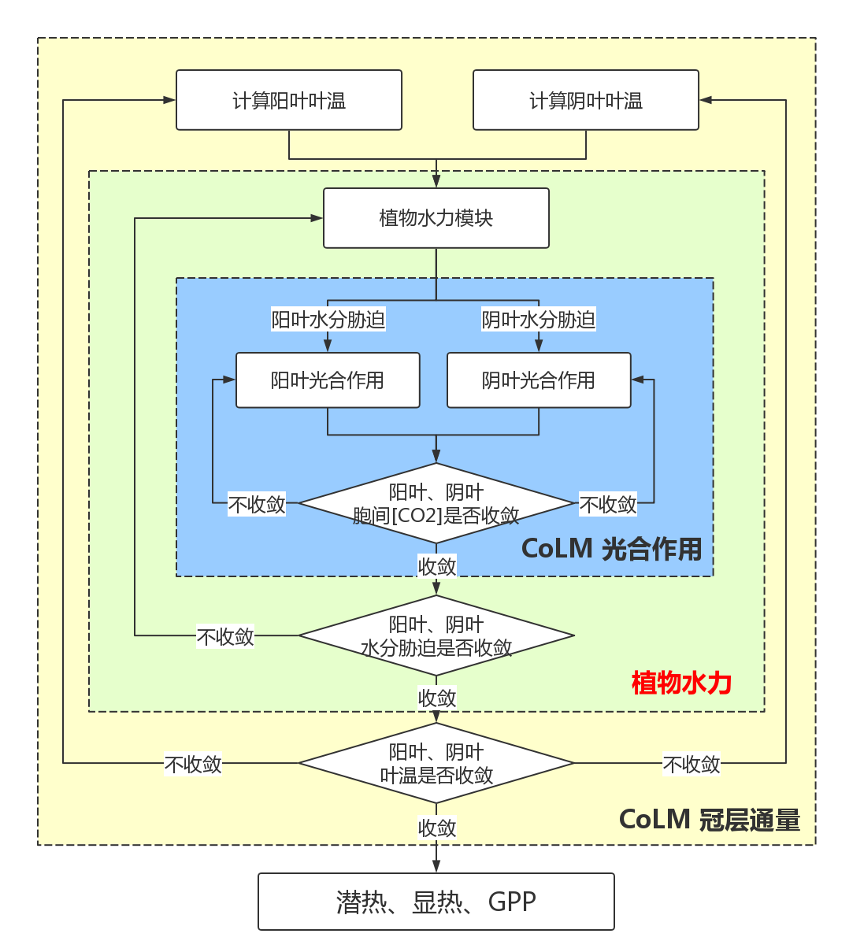
\includegraphics{Figures/植被水力模式/植被水力模式的数值模拟流程图.png}
    \caption{植被水力模式的数值模拟流程图。}
    \label{fig:植被水力模式的数值模拟流程图}
    \end{figure}
}

